\documentclass[parskip=full]{scrartcl}
\usepackage[utf8]{inputenc} % use utf8 file encoding for TeX sources
\usepackage[T1]{fontenc}    % avoid garbled Unicode text in pdf
\usepackage[english]{babel}  % english hyphenation, quotes, etc
\usepackage[colorlinks=true,linkcolor=blue]{hyperref}       % detailed hyperlink/pdf configuration
\usepackage{graphicx}       % provides commands for including figures
\usepackage{csquotes}       % provides \enquote{} macro for "quotes"
\usepackage{enumitem}
\usepackage{multicol}
\setlength{\columnsep}{4cm}
%\usepackage{lscape}	% provides landscape portrait

\usepackage{pdflscape}	% provides horizental landscape portrait


\usepackage{pdfpages}	% add another pdf in  Latex

\usepackage{tikz}


\usepackage{verbatim}	% provides multi-line comments

\usepackage{afterpage}
\usepackage{ragged2e}
\usepackage[export]{adjustbox}
\newcommand\tab[1][1cm]{\hspace*{#1}}


\title{\Huge \textbf{HePICS Deployment-Phase Document}}
\date{\today \vspace{+10ex}}
\author{Andres Stober \\
	\and Mehyar Cherni \\
	\and Ibrahim Bouriga \\ 
	\and Linjuan Fan \\
	\and Bahaa Mahagne \\ }

\begin{document}

\maketitle
\thispagestyle{empty}

\begin{tikzpicture}[remember picture, overlay]
  \node [anchor=north west, inner sep=0.5pt, yshift=-20pt,xshift=20pt]  at (current page.north west)
     {
\includegraphics[height=1.9cm]{Logo_KIT}};
\end{tikzpicture}

\begin{figure}[b]
\centering
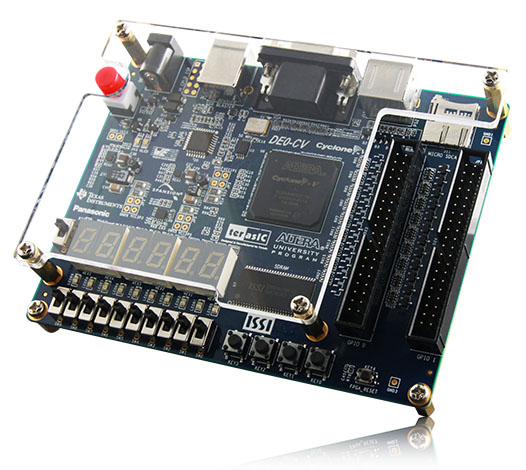
\includegraphics[width=0.45\textwidth, center]{boardimage}
\end{figure}

\pagebreak

\tableofcontents
\thispagestyle{empty}
\pagebreak

\section {Introduction : HePICS}
HePICS stands for Heterogeneous Platform for an Image Classification System, which was the task of this software engineering practise.\\
The software employs the topology of the AlexNet artificial neural network in order to classify images. For this purpose, it offers the user the possibility of choosing one or multiple images, enabling the platforms it is designed to run on, as well as the operation mode. Besides, it contains the feature of aggregating the results of different classifications.\\
A user inteface has been designed to make the contact with the software easier and its use more appealing. Every step the user has to take to properly run the classification is lead to by a button .\\
The software only enables the classification through a cpu for the moment, which means the choice of the mode doesn't have any influence on the performance. The classification of a single image lasts in average around 4,6 seconds. Although running on the fpga should theoretically increase the performance.\\
The progressbar gives an estimation about the duration of the classification of all input images, and after testing different use cases, the software has been proven to be in a stable state and to run as expected.


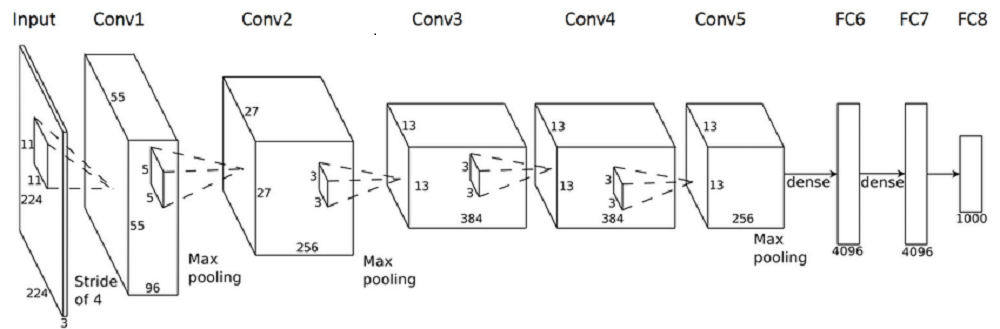
\includegraphics[width=0.9\textwidth, center]{topology}


\pagebreak
 
\section {Software Engineering as A Practise}
Software engineering is a practise which sets the rules for each individual or group who is willing to develop a software product. During the development of HePICS, the waterfall model has been followed, which leads us to this final phase : the release, or deployment. It has been made sure that the common knowledge of software engineering was applied during every phase, was it analyzing the requirements, designing and implementing the structure or testing it, or even version control. To read about these practises seems like any other knowledge, but to perform them has proven to be a harder task than expected, and definitely an interesting experience. As a matter of fact, besides object oriented programming, we had to explore every corner of the waterfall model, from UML diagrams to unit tests and deployment, the idea around software engineering has been made clearer.


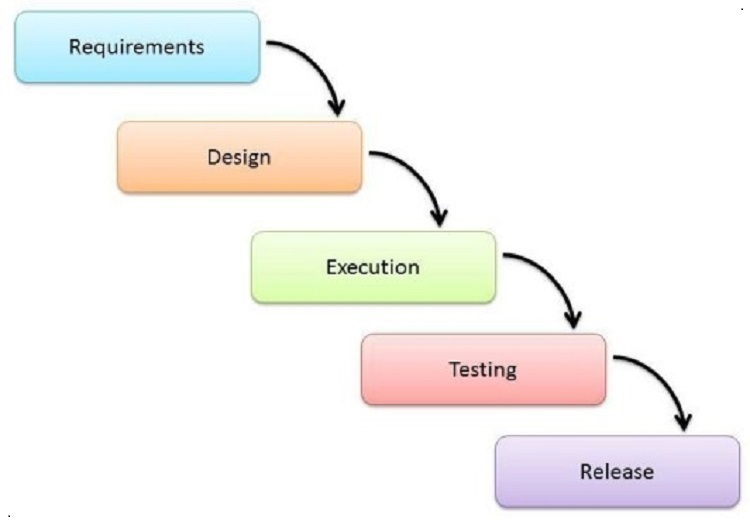
\includegraphics[width=0.80\textwidth, center]{swt}


\pagebreak

\section {Functionality Description}
The following only describes the general structure of the program, and the major changes made after the design phase.\\
The program implements with the help of the caffe library an AlexNet neural network. The network is generated automatically through the configuration file when the program is run. It contains an array of layers set in the right order of the topology. Possible layer types are convolutional, normal response normalization, maxpool, or  fully connected. The activation functions have also been implemented as layers in order to make the design of a pipeline possible.  \\
The GUI takes the input from the user and passes it through the Assistant, Scheduler and DataSaver to the system. The Classifier takes then each input and passes it through the layers' pipeline, which produces a result to display on the user interface.
If the fpga is enabled, the classifier should run the convolutional layer on it. Unfortunately, its implementation couldn't be accomplished in time. 


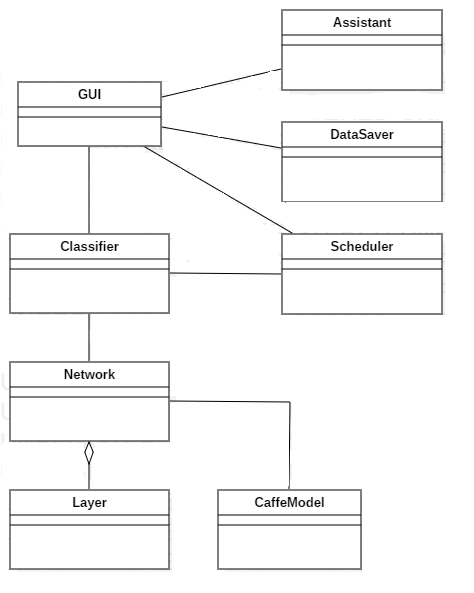
\includegraphics[width=0.60\textwidth, center]{diagram}

\pagebreak

\section {Implementation Challenges}
Due to the group being unfamiliar with the concept of a neural network, loading images correctly has proven to be quite the challenge. The first interpretation was a simple 2D vector, but we slowly figured out it wasn't enough since the convlutional layer needs more paremeters for it to apply its filter. While refactoring the program and trying to code a cleaner design after the implementation phase, the image was represented as a 3D model.
\\ The program has been able to run since then, but with wrong results. While debugging, errors in the implementation of some  layers were uncovered, but the major issue has been figured with the help of the caffe model. In fact reading its implementation and following each step of it has been nothing but helpful to the process of correctly interpreting the classification. \\
Another task that turned out to be a bit challenging was the the use of external libraries on eclipse, as it demands more steps than library integration with programming languages we're familiar with. 

\section {Libraries and Tools}
Eclipse was used to manage the project and building it, however QtCreator was also used to design the user interface. Both were later integrated on eclipse. \\
These are the libraries used in the program :

\begin{itemize}
	\item Qt5Gui : contains the QImage class which was used to read and load images.
	\item Qt5Core : contains the QString class which is necessary to specify the input path 
	\item Qt5Widgets : contains the classes necessary for creating a graphical user interface 
	\item Protobuf : used to serialize strcutured data 
	\item Caffe : served as a parser for the neural network and generated the weight file.
	\item GoogleTest : provided unit testing functions
\end{itemize}

\pagebreak

\section {Requirements Check}
\subsection {Must requirements}
The following must requirements have been fulfilled.
\begin{itemize}
	\item The system must be able to classify images.
	\item The system must allow the selection of one or more input images.
	\item The system must show the result of the treatment.
	\item The system must employ artificial neural networks.
	\item The system must deploy the AlexNet deep neural network.
	\item The system must know at least one set of weights.
	\item The system must offer three performance profiles : 
	\begin{itemize}
		\item High Performance
		\item Low Power
		\item Energy Efficency
	\end{itemize}
	\item The system must allow the control and the execution of commands through a GUI interface.
	\item The system must be able to run the GUI on an Ubuntu system.
	\item The system must exhibit a classification interface.
	\item The system must include the aggregate feature. This feature fuses the results of different treatments of the same object in order to reach more precision.
	\item The system must offer the possibility of entering up to 5 images in the aggregate feature.
\end{itemize}
\pagebreak

The following must requirements have not been fulfilled.
\begin{itemize}
	\item The system must be able to execute intense calculations through heterogeneous platforms (CPU, GPU, FPGA, ASIC).
	\item The system must support an FPGA through OpenCL.
	\item The system must hide the OpenCL details behind an abstraction layer.
	\item The system must be able to measure its performance.
	\item The system must be able to measure its power consumption.
	\item The system communicate with another system. It looks into a file to search for an image treatment request, and send back the results via Ethernet connection.
\end{itemize}
\subsection {Can requirements}
The following can requirements have been fulfilled.
\begin{itemize}
	\item The system can offer the possibility of entering more than 5 images in the aggregate feature.
	\item The system can run batch processing.
	\item The system can pause, resume or cancel the classification process.
	\item The system can beautify the output result.
\end{itemize}

\pagebreak
	
\section {Statistics}
The following presents some numbers and statistics about the project's implementation and testing.
\begin {itemize}
	\item Lines of code : around 3400 in total, around 500 lines of comments or whitespaces
	\item Branches : Master which contains the presentations and documents + old code, another 13 branches which served to the integration, or individual work
	\item Commits : 340
	\item Tests : 15 Test classes were written, leading to more than 30 test cases
	\item Coverage : reached an overall of 68 \% 
\end {itemize}
Most parts which weren't tested are either very simple implementations, dead code, or exception handling. Some of these have been manually tested, however, every layer and functions which are to heavily to rely on have been properly tested.

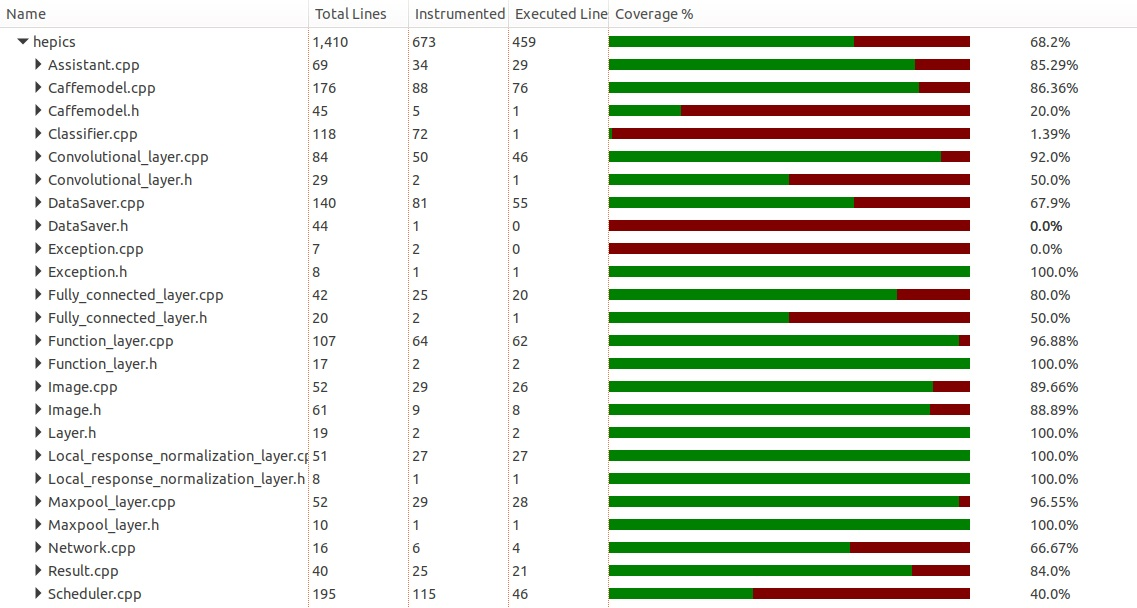
\includegraphics[width=1.2\textwidth, center]{hepics_coverage}


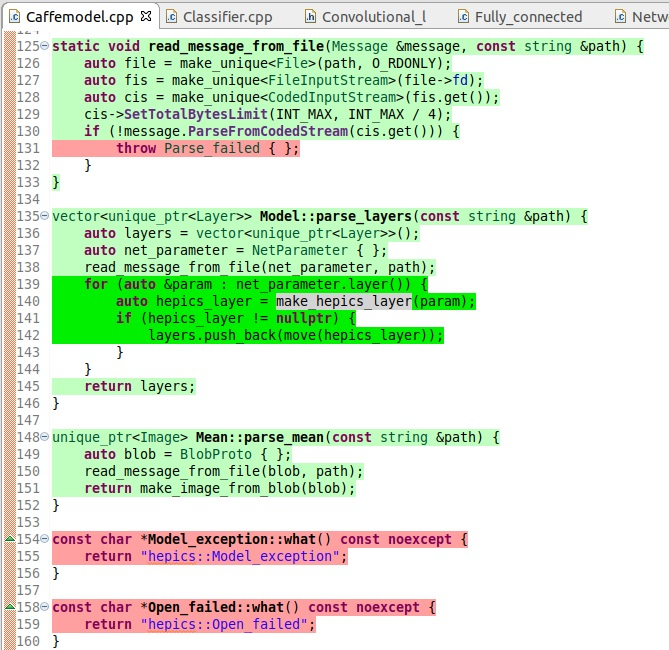
\includegraphics[width=1\textwidth, center]{error_code}


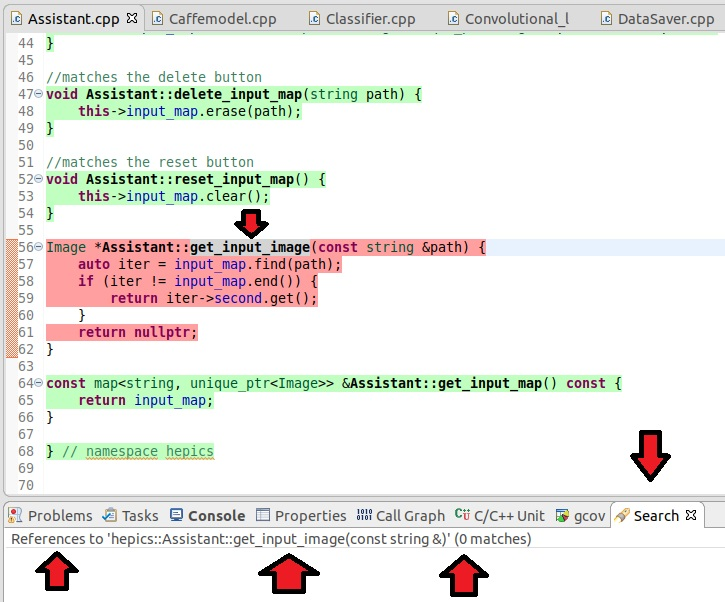
\includegraphics[width=1\textwidth, center]{dead_code}

\pagebreak

\section {Readme and Installation}
To download the package, please run the following command in the terminal : \\
scp pselab1819@141.3.77.54:~/hepics.tar.gz hepics.tar.gz \\
password : pselab1819 \\
Once the package has been unzipped, please refer to the instructions in the readme file.\\
Installation :

\begin{itemize}
	\item sudo apt-get install libprotobuf-dev protobuf-compiler
	\item  sudo apt-get install build-essential
	\item sudo apt-get install qtcreator 
	\item sudo apt-get install qt5-default
	\item make all
	\item hepics
\end{itemize}

\section {Screenshots}
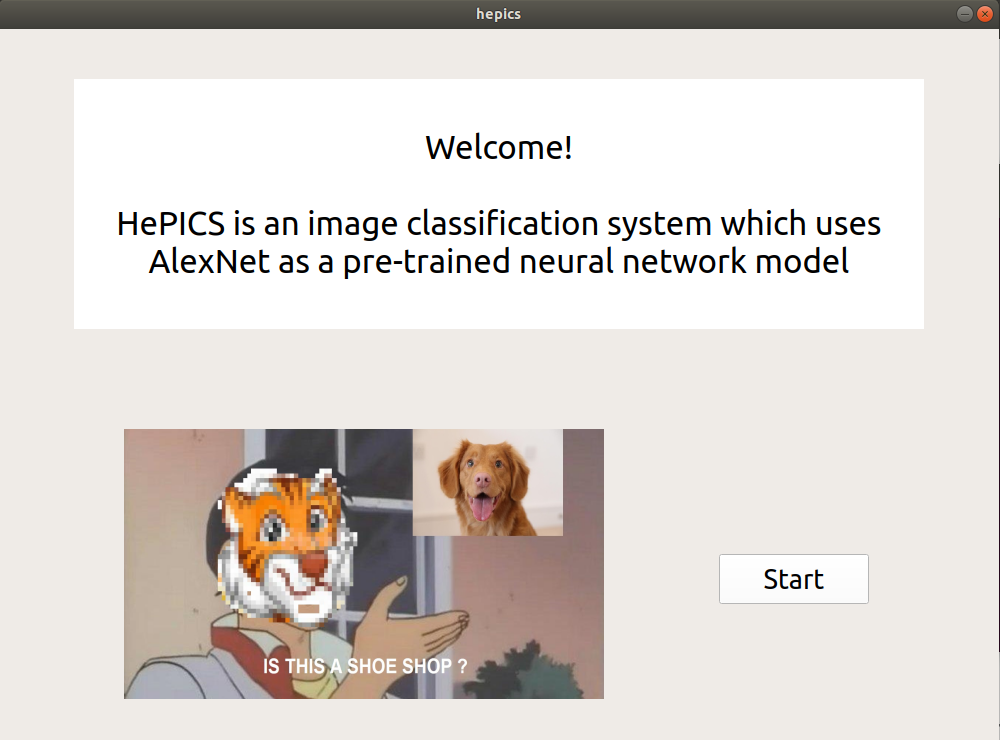
\includegraphics[width=0.80\textwidth, center]{screen1}
\pagebreak
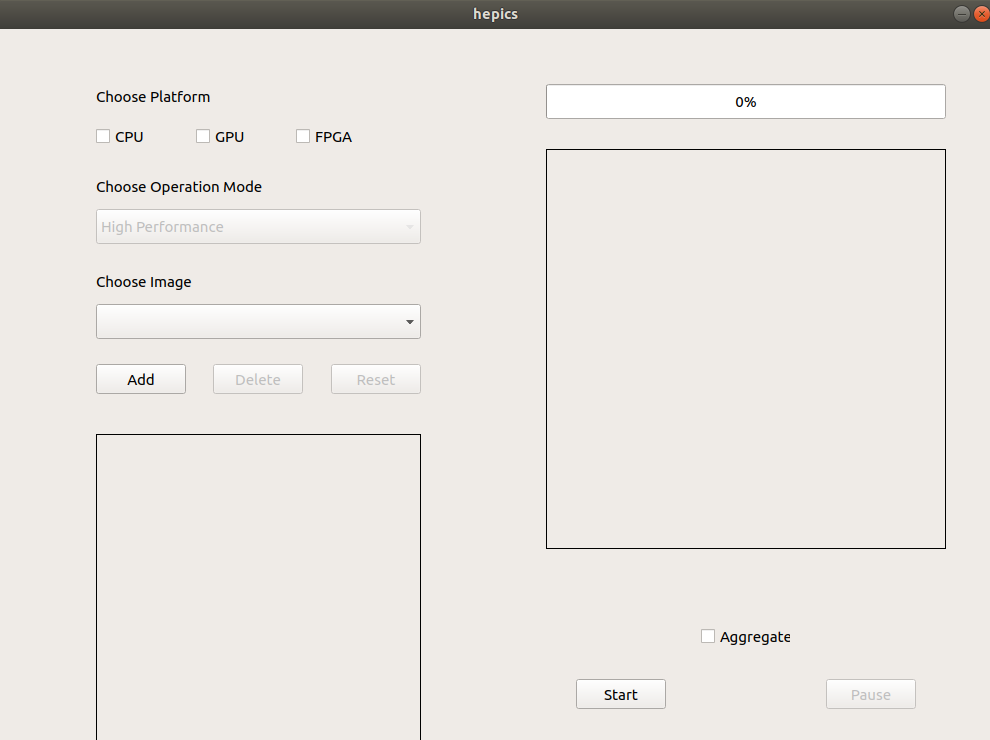
\includegraphics[width=0.80\textwidth, center]{screen2}
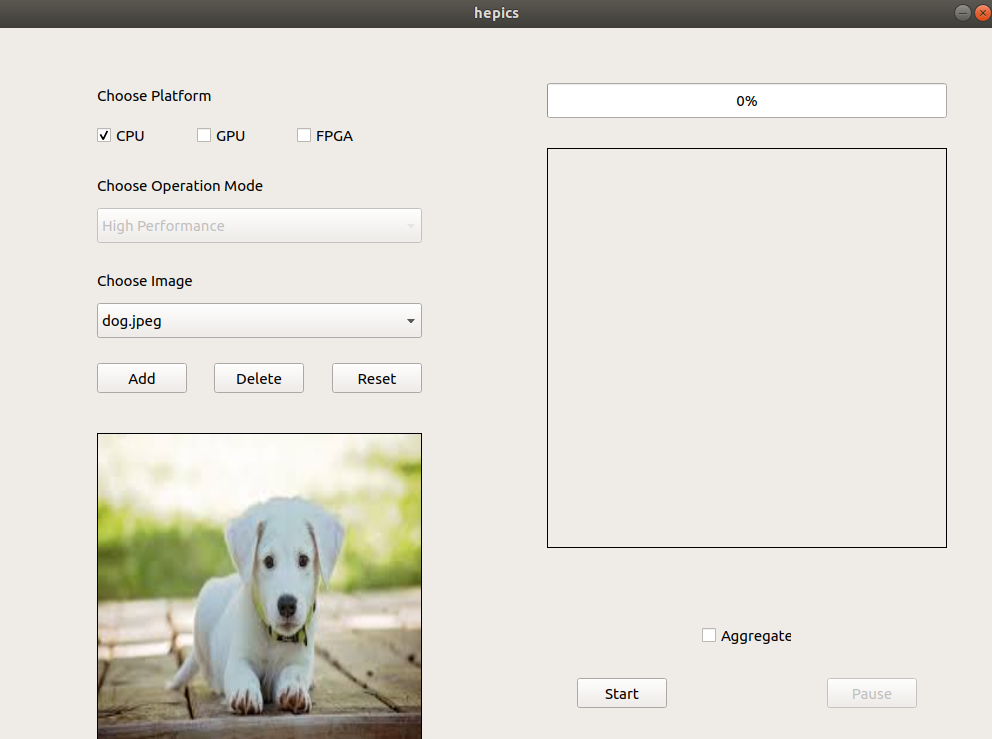
\includegraphics[width=0.9\textwidth, center]{screen3}
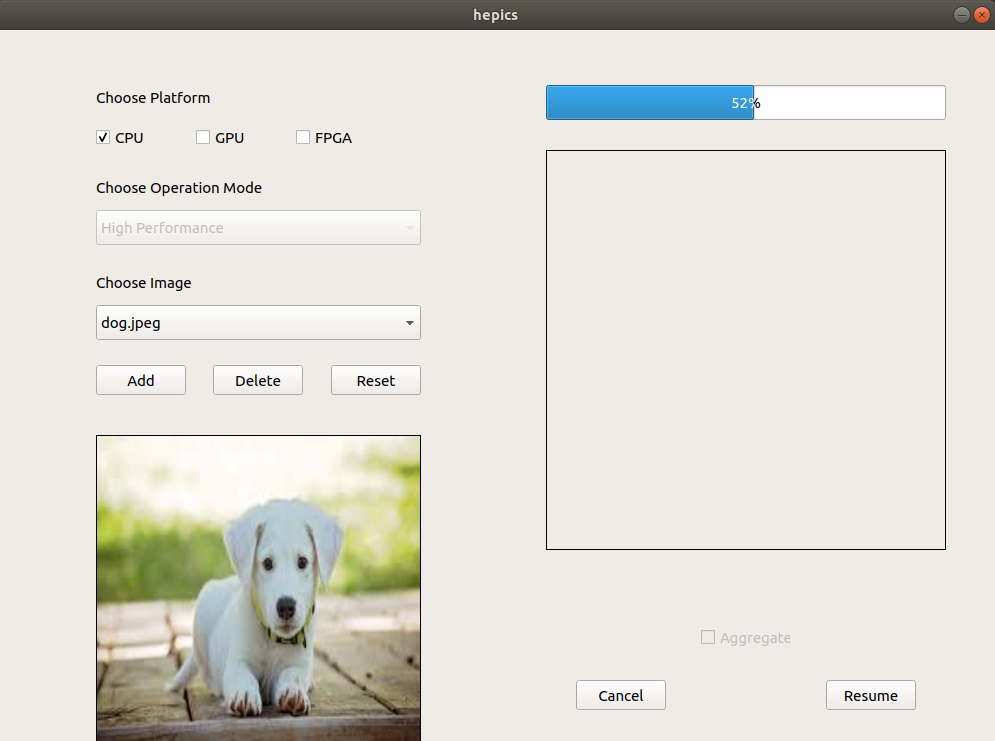
\includegraphics[width=0.9\textwidth, center]{screen4}
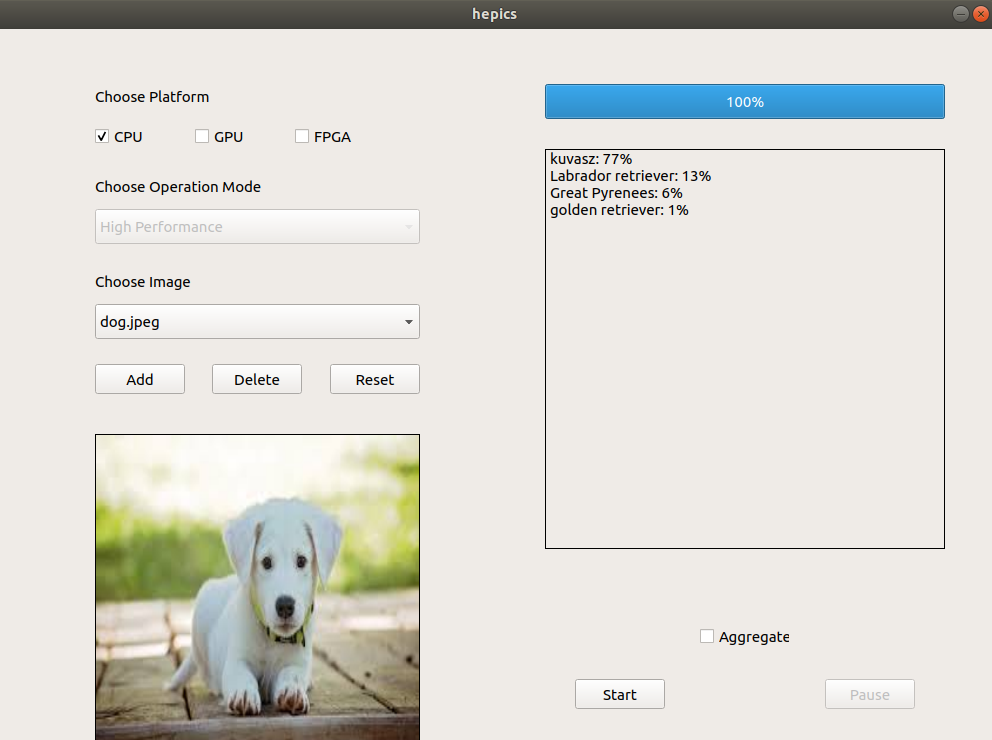
\includegraphics[width=0.9\textwidth, center]{screen5}
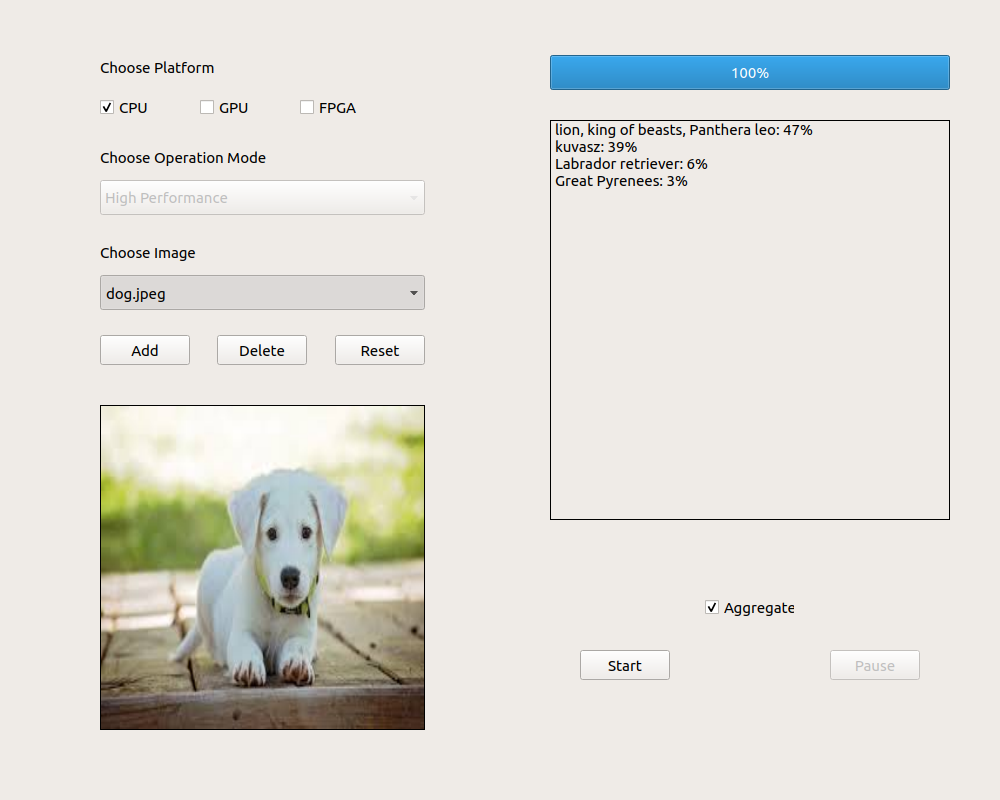
\includegraphics[width=0.9\textwidth, center]{screen6}
\end{document}